\documentclass[12pt]{article}
\usepackage{enumitem}
\usepackage{mathtools}
\usepackage{amsthm}
\usepackage{graphicx}
\graphicspath{ {images/} }
\begin{document}

\title{Assignment 9}
\author{Darwin Ding}
\maketitle

\section*{1. 8th order Polynomial Feature Transform}
Each data point creates two features (symmetry and intensity were chosen for this assignment), and the total 8th order polynomial transform using Legendre transforms increases each point to 45 dimensions. Therefore, the training set $Z$ is \textbf{300 x 45}.

\section*{2. Overfitting}
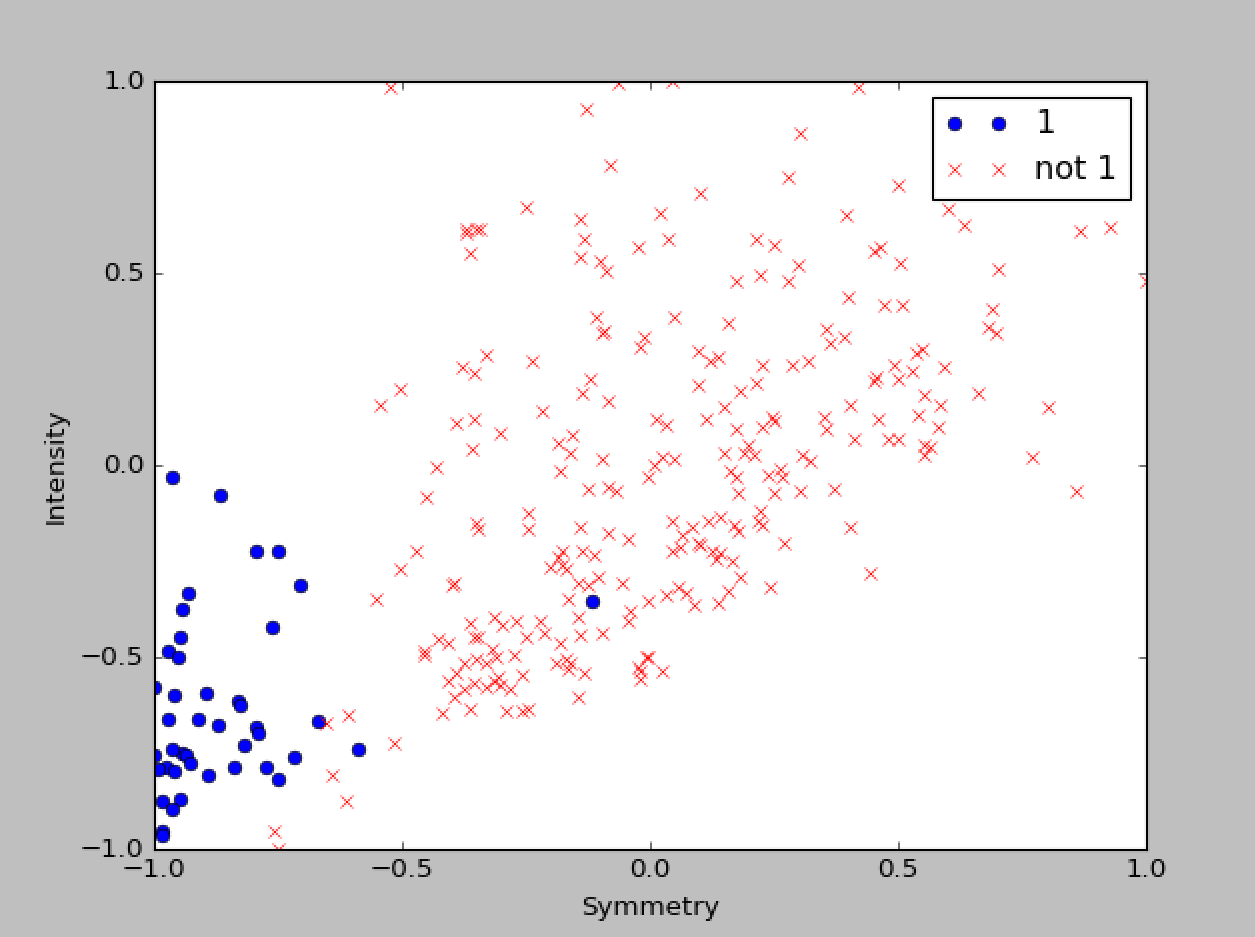
\includegraphics[scale=.5]{2-2.png}

This is the original plot of all the data points. It is pretty clear where you can draw a line in order to have a pretty decent $E_{in}$. It's not linearly separable data, but you can't always have that in the real world.

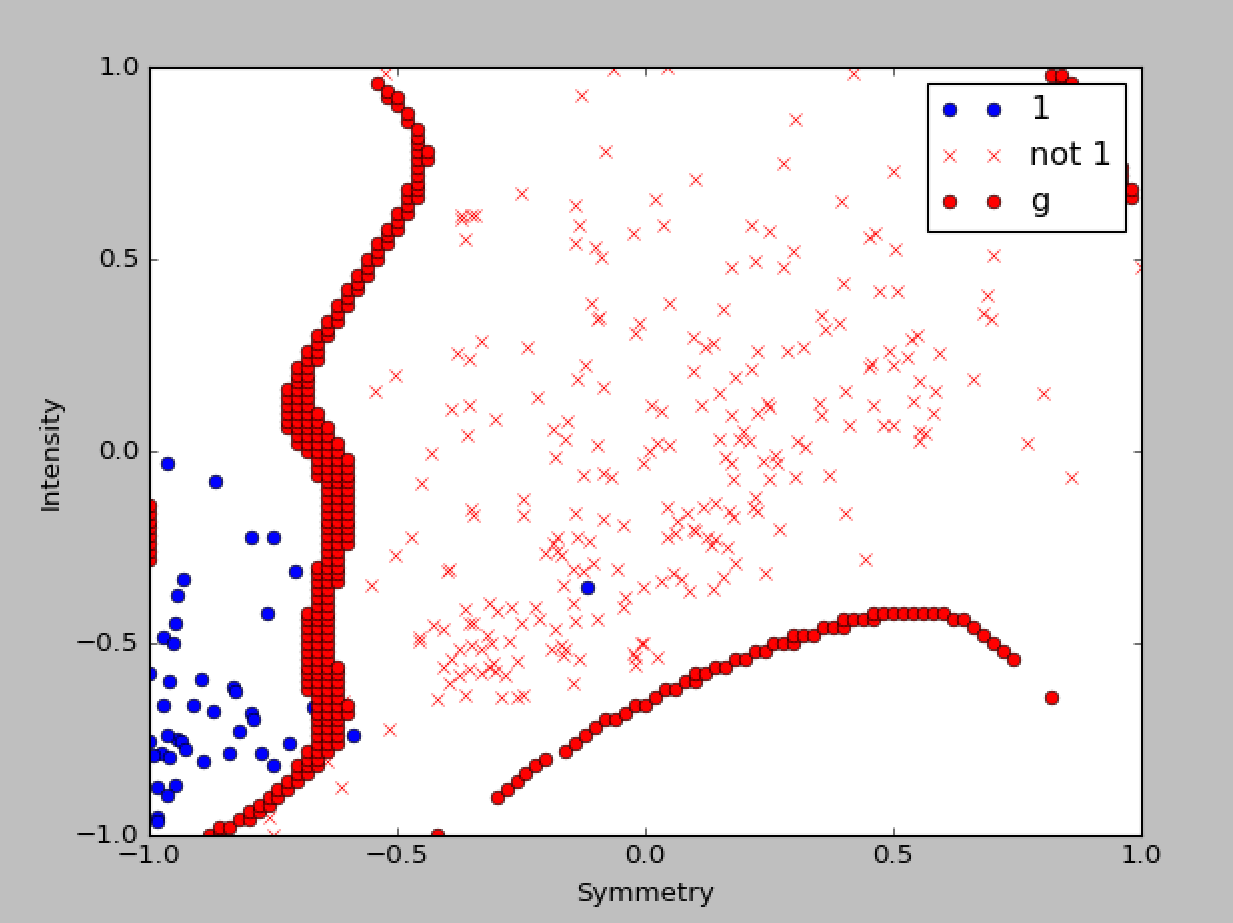
\includegraphics[scale=.5]{2-1.png}

This is the plot with the model without any regularization. As you can see, there is quite a bit of overfitting here. In order to conform with the shape of the 1s, the algorithm outputs a bound that flows with the data points a little bit too much for our comfort. The red dots represent the outputted hypothesis. Also note the large curve on the bottom that's only possible due to a gap in the "not 1" points. We would probably not expect points in this region to actually be considered 1s in real life.

\section*{3. Regularization}
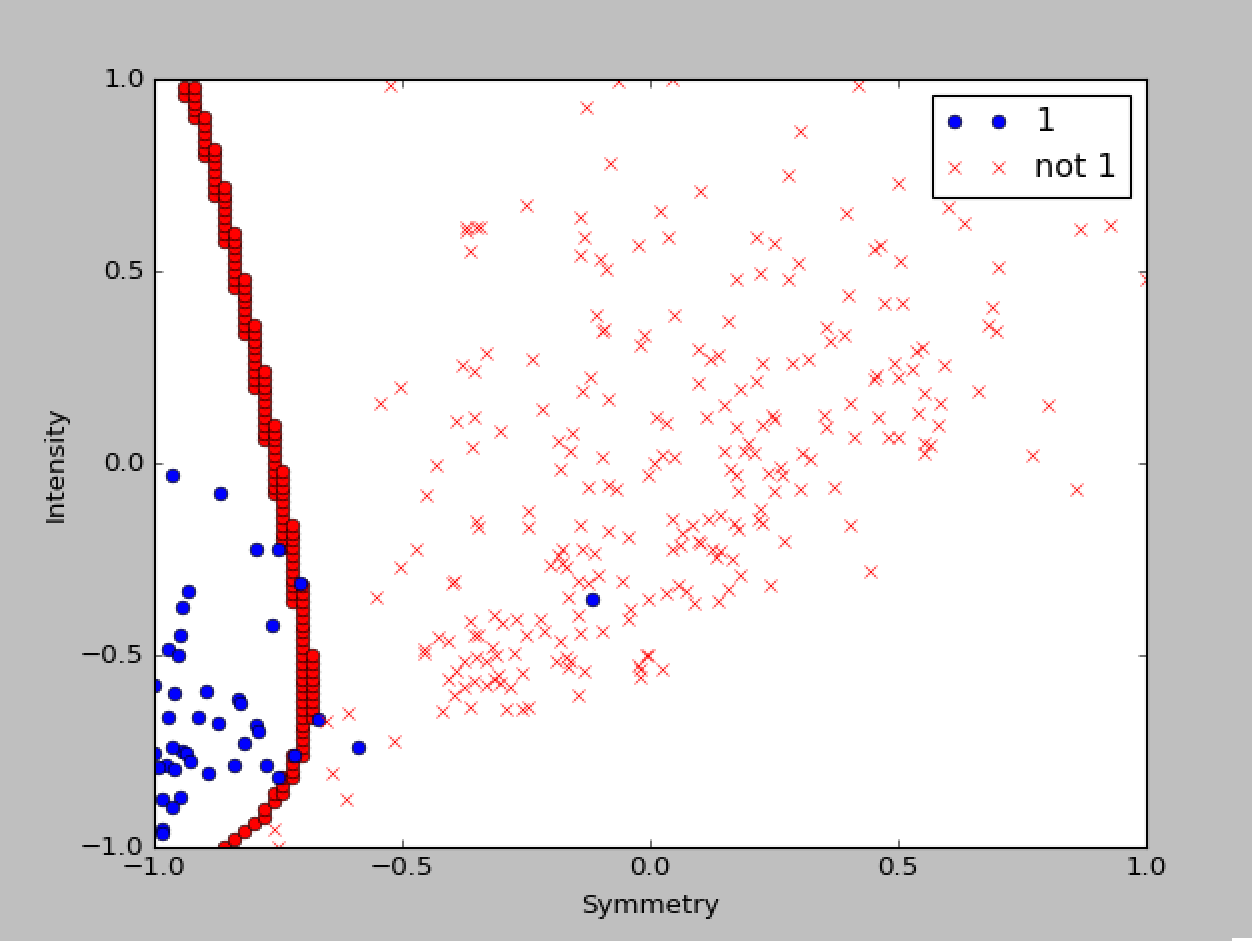
\includegraphics[scale=.5]{3-1.png}

There is a tinge of underfitting here. Notice the blue points that are to the right of the red curve that could be added to the left side of the curve without any loss in $E_{in}$. This is typically a sign that we're probably doing a little too much regularization.

\section*{4. Cross Validation}
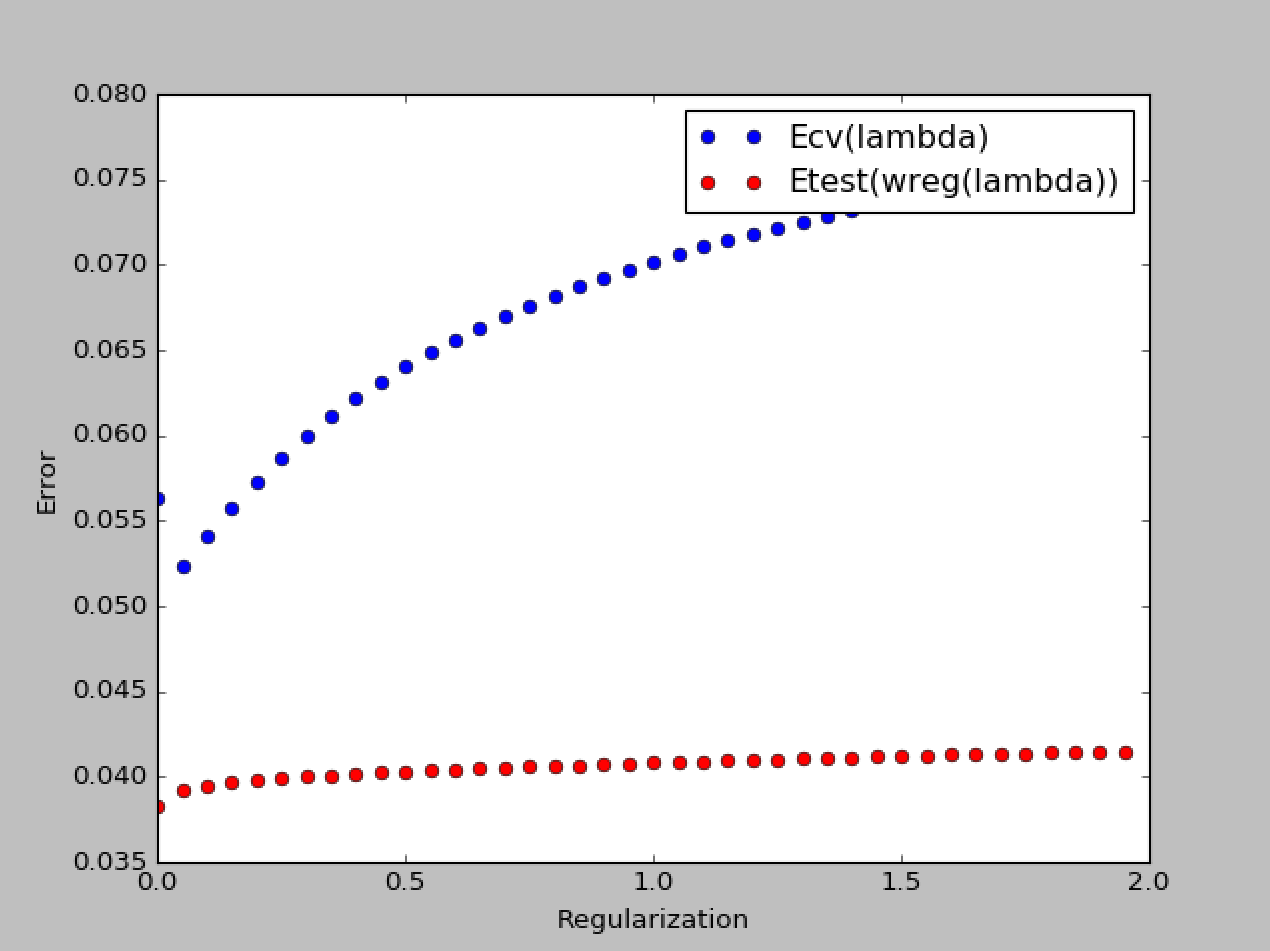
\includegraphics[scale=.5]{4-1.png}

Note that I had to start the regularization constant from 0.001 instead of from 0, because the $E_{test}$ at 0 was returning an extremely high value that was skewing the entire graph. On the graph above, imagine there is a red point all the way above the graph at $(0, 1.88)$.

At first, $E_{cv}$ starts at a value when $\lambda = 0$ and goes down initially as you increase regularization. This is because some amount of regularization is very important to make sure that you aren't totally overfitting the data with some crazy curves. However, as you continue to increase regularization, you underfit the data by overconstraining your hypotheses, and your $E_{test}$ and $E_{cv}$ will increase.

\section*{5. Pick $\lambda$}
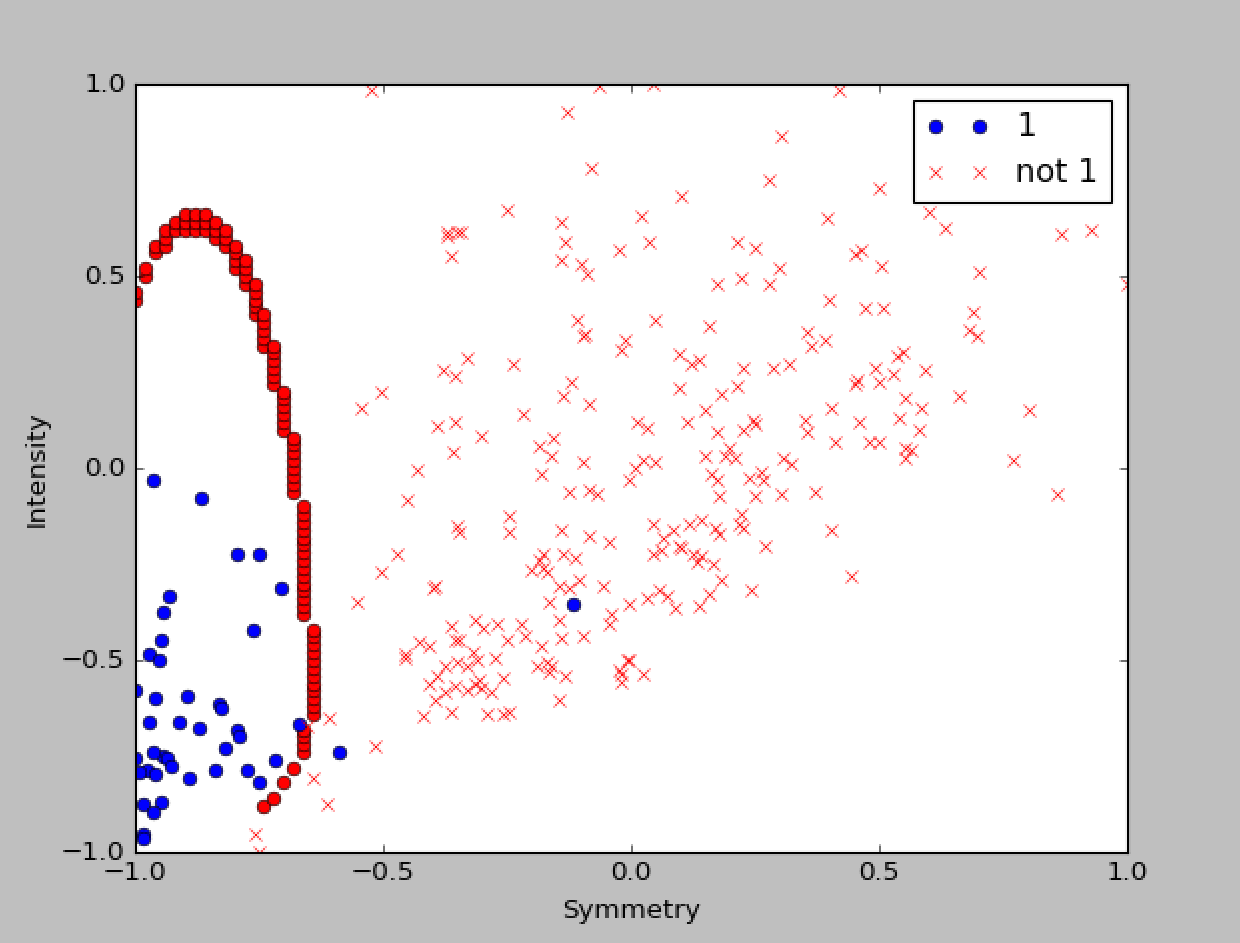
\includegraphics[scale=.5]{5-1.png}

The minimum $E_{cv}$ was found at $\lambda = 0.014$, and the resulting weights created the above separation. This is a pretty good boundary, as it's quite accurate and does not have complicated curves.

\section*{6. Estimate $E_{out}$}
Running the weights generated from a regularization of $0.014$ resulted in an $E_{out}$ of \textbf{0.0388}. This is a very decent estimate!

\section*{7. Is $E_{cv}$ biased?}
No it is not biased! We did not touch the test set, so our $E_{cv}(\lambda^*)$ estimates will estimate out $E_{test}$ estimates quite well.

\section*{8. Data snooping}
However, we are guilty of unconscious data snooping. When we originally scaled and normalized, we did so before removing data for the test set. As a result, our results were unintentionally dependent on the test set, and we have a biased estimate of $E_{out}$. Fortunately, if we remove for the test set then run our learning algorithm, we can circumvent this.

\end{document}